\documentclass[crop,tikz]{standalone}
\usepackage{pgfplots}
\pgfplotsset{compat=1.18}

% Field lines and lines of constant potential for a plate with
% infinite length (along the z-axis) and finite width in x direction.
%
% Inspired by the expressions given in Maxwell's "A treatise on
% electricity and magnetism" XII.192 Example V and Fig. X.

\pgfplotsset{
  inverted/.style = {
    every axis legend/.append style={
      draw=white,
      fill=hardblack,
      text=white
    }
  },
}

\begin{document}
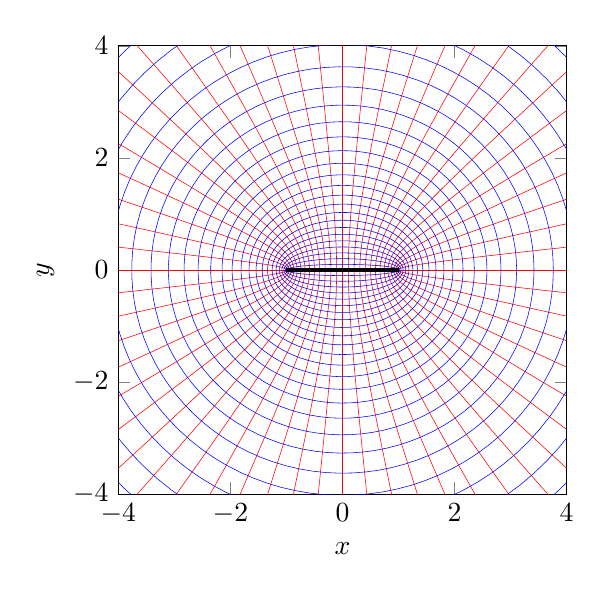
\begin{tikzpicture}
  \pgfmathsetmacro{\numberoffieldlines}{30};
  \pgfmathsetmacro{\numberofpotentiallines}{30};
  \pgfmathsetmacro{\platesize}{1};
  \pgfmathsetmacro{\psimin}{0}; % minimum psi
  \pgfmathsetmacro{\psimax}{pi}; % maximum psi
  \pgfmathsetmacro{\phimin}{0}; % minimum phi
  \pgfmathsetmacro{\phimax}{3}; % maximum phi
  \pgfmathsetmacro{\remin}{-4*\platesize};
  \pgfmathsetmacro{\remax}{-\remin};
  \pgfmathsetmacro{\immin}{-4*\platesize};
  \pgfmathsetmacro{\immax}{-\immin};
  \begin{axis}[
    axis equal image,
    xmin={\remin}, xmax={\remax},
    ymin={\immin}, ymax={\immax},
    xlabel={$x$},
    ylabel={$y$},
    samples=100,
    declare function = {
      fx(\x,\y) = cosh(\x)*cos(deg(\y));
      fy(\x,\y) = sinh(\x)*sin(deg(\y));
      phi(\n,\nmax) = \phimin + \n/\nmax*(\phimax - \phimin); % ulates phi
      psi(\n,\nmax) = \psimin + \n/\nmax*(\psimax - \psimin); % ulates psi
    },
    ]
    % field lines
    \pgfplotsinvokeforeach{0,...,{\numberoffieldlines}}{
      \addplot[red,very thin,domain={\remin}:{\remax}] (
        {\platesize*fx(x,psi(#1,\numberoffieldlines))},
        {\platesize*fy(x,psi(#1,\numberoffieldlines))}
      );
    }
    % lines of constant potential
    \pgfplotsinvokeforeach{0,...,{\numberofpotentiallines}}{
      \addplot[blue,very thin,domain=0:{2*pi}] (
        {\platesize*fx(phi(#1,\numberofpotentiallines),x)},
        {\platesize*fy(phi(#1,\numberofpotentiallines),x)}
      );
    }
    % plate
    \addplot[domain={-\platesize}:{\platesize},ultra thick] {0};
  \end{axis}
\end{tikzpicture}
\end{document}
